\begin{name}
	{\tenchude}
	{\tendethi}
	{\tentruong}
	{\thoigian}
\end{name}
\setcounter{ex}{0}\setcounter{bt}{0}
\TN
\Opensolutionfile{ans}[ans/ansDe5-TN5]
\begin{ex}%[EX-TF-TLN-2024-ĐỢT 2, Trần Lệnh Ánh]%[2D1N1-1]
	Xét mẫu số liệu ghép nhóm được cho ở bảng sau
	\begin{center}
		\begin{tabular}{|l|c|c|c|c|c|}
			\hline Nhóm   & {$\left[a_1; a_2\right)$} & $\ldots$ & {$\left[a_i; a_{i+1}\right)$} & $\ldots$ & {$\left[a_k; a_{k+1}\right)$} \\
			\hline Tần số & $m_1$                     & $\ldots$ & $m_i$                         & $\ldots$ & $m_k$                         \\
			\hline
		\end{tabular}
	\end{center}
	Nếu $m_1$ và $m_k$ cùng khác $0$ thì khoảng biến thiên của mẫu số liệu ghép nhóm được tính theo công thức
	\choice
	{\True $R=a_{k+1}-a_1$}
	{$R=a_{2}-a_1$}
	{$R=\dfrac{a_{k+1}+a_1}{2}$}
	{$R=a_{k+1}-a_k$}
	\loigiai{
	Khoảng biến thiên của mẫu số liệu ghép nhóm được tính theo công thức $R=a_{k+1}-a_1$.
	}
\end{ex}

\begin{ex}%[2D1N1-2]%[CTST - Lớp 12 - Ôn tập cuối học kì 1 - Đề 2]%[Nguyễn Văn Sang]
	Cho hàm số $y=f(x)$ có bảng biến thiên sau
	\begin{center}
		
\begin{tikzpicture}[scale=1, font=\footnotesize, line join=round, line cap=round, >=stealth]
			\tkzTabInit[nocadre=false,lgt=1,espcl=2,deltacl=0.5]
			{$x$/.7 ,$y'$/.7,$y$/2}
			{$-\infty$ , $-1$ , $1$ , $+\infty$}
			\tkzTabLine{ , + , $0$ , - , $0$ , + , }
			\tkzTabVar{-/$-\infty$ , +/$3$ , -/$-2$ , +/$+\infty$}
		\end{tikzpicture}
	\end{center}
	Hàm số đã cho đồng biến trên khoảng nào sau đây
	\choice
	{\True $(1 ;+\infty)$}
	{$(-1 ; 1)$}
	{$(-1 ;+\infty)$}
	{$(-\infty ; 1)$}
	\loigiai{
		Từ bảng biến thiên ta thấy, trên $(1 ;+\infty), y'>0$ nên hàm số đồng biến trên $(1 ;+\infty)$.}
\end{ex}

\begin{ex}%[2D1V1-5]%[Tổ 16 - Đợt 16 - Chương 1 - - KNTT - Đề 3]%[Nguyễn Kiều Nhã Tú]
	Để giảm nhiệt độ trong phòng từ $28^{\circ}\mathrm{C}$, một hệ thống làm mát được phép hoạt động trong $10$ phút. Gọi $T$ (đơn vị $^\circ \mathrm{C}$) là nhiệt độ phòng ở phút thứ $t$ được cho bởi công thức $T=-0,008 t^3-0,16 t+28$ với $t \in[1 ; 10]$. Trong thời gian $10$ phút kể từ khi hệ thống làm mát bắt đầu hoạt động, nhiệt độ trong phòng tăng hay giảm?
	\choice
	{Tăng}
	{\True Giảm}
	{Tăng rồi giảm}
	{Giảm rồi tăng}
	\loigiai{
		Xét hàm số $T=-0,008 t^3-0,16 t+28$ với $t \in[1 ; 10]$.\\
		Ta có $T^{\prime}=-0,024 t^2-0,16<0, \forall t \in[1 ; 10]$.\\
		Suy ra hàm số $T$ nghịch biến trên đoạn $[1 ; 10]$ nhiệt độ trong phòng giảm.
	}
\end{ex}

\begin{ex}%[Mức độ N]%[2D1N2-1]
	Hàm số nào dưới đây không có cực trị?
	\choice{$y=\dfrac{x^2+1}{x}$}{\True $y=\dfrac{2x-2}{x+1}$}{$y=x^2-2x+1$}{$y=-x^3+x+1$}
	\loigiai{Xét hàm số $y=\dfrac{2x-2}{x+1}\text{, } \forall x \ne-1$.\\ Ta có $y'=\dfrac{4}{(x+1)^2}>0\text{, } \forall x \ne -1$.\\
		Vậy hàm số $y=\dfrac{2x-2}{x+1}$ không cực trị.}
\end{ex}

\begin{ex}%[2D1N2-2]%[CD - Lớp 12 - Ôn tập cuối học kì 1 - Đề 5]%[Đoàn Thị Lý]
	\immini[thm]{
		Cho hàm số $y=f(x)$ có đồ thị như hình vẽ bên. Điểm cực tiểu của hàm số đã cho là
		\choice
		{$x=-1$}
		{$x=2$}
		{$x=3$}
		{\True $x=0$}
	}
	{
		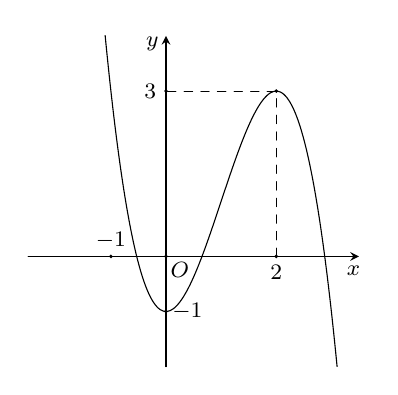
\begin{tikzpicture}[scale=0.7, font=\footnotesize, line join=round,	line cap=round, >=stealth]
			\def \xmin{-2.5}
			\def \xmax{3.5}
			\def \ymin{-2}
			\def \ymax{4}
			\draw[->] (\xmin,0)--(\xmax,0) node[shift=(-110:0.2)] {$x$};
			\draw[->] (0,\ymin)--(0,\ymax) node[shift=(-150:0.2)] {$y$};
			\fill (0,0) circle(1pt) node[shift=(-45:0.25)]{$O$}
			(-1,0) circle(1pt) node[shift=(90:0.2)]{$-1$}
			(2,0) circle(1pt) node[shift=(-90:0.2)]{$2$}
			(0,-1) circle(1pt) node[shift=(0:0.27)]{$-1$}
			(0,3) circle(1pt) node[shift=(180:0.2)]{$3$} (2,3) circle(1pt);
			\draw[dashed] (2,0)|-(0,3);
			\clip (\xmin,\ymin) rectangle (\xmax,\ymax);
			\draw[smooth,samples=100,domain=\xmin:\xmax,xshift=1cm] plot(\x,{-(\x)^3+3*(\x)+1});
		\end{tikzpicture}
	}
	\loigiai{
		Từ đồ thị suy ra điểm cực tiểu của  hàm số đã cho là $x=0$.
	}
\end{ex}

\begin{ex}%[Mức độ H]%[2D1H2-1]
	Cho hàm số $y=\dfrac{x^2+3}{x+1}$. Mệnh đề nào dưới đây đúng?
	\choice{Giá trị cực tiểu của hàm số bằng $-3$}{Giá trị cực tiểu của hàm số bằng $1$}{Giá trị cực tiểu của hàm số bằng $-6$}{\True Giá trị cực tiểu của hàm số bằng $2$}
	\loigiai{Ta có $y'=\dfrac{x^2+2x-3}{(x+1)^2}$; $y'=0\Leftrightarrow x^2+2x-3=0\Leftrightarrow \left[\begin{array}{l}
			x=-3 \\x=1.
		\end{array}\right.$\\
	Bảng biến thiên
	\begin{center}
		
\begin{tikzpicture}
			\tkzTabInit[nocadre=false, lgt=1.5,espcl=3.5]
			{$x$/1,$y'$/1,$y$/2}
			{$-\infty$,$-3$,$-1$,$1$,$+\infty$}
			\tkzTabLine{,+,0,-,d,-,0,+, }
			\tkzTabVar{-/$-\infty$,+/$-6$,-D+/$-\infty$/$+\infty$,-/$2$,+/$+\infty$/}
		\end{tikzpicture}
	\end{center}
	Vậy hàm số đạt cực tiểu tại điểm $x=1$ và giá trị cực tiểu bằng $2$.}
\end{ex}

\begin{ex}%[2D1H3-1]
	Tìm giá trị nhỏ nhất của hàm số $y = 2\cos^2 x - 3\cos x + 1$ trên tập xác định $\mathbb{R}$.
	\choice
	{$\dfrac{1}{3}$}
	{$\dfrac{1}{4}$}
	{\True $-\dfrac{1}{8}$}
	{Không tồn tại}
	\loigiai{
		Đặt $t = \cos x$, $t \in [-1;1]$. Khi đó hàm số trở thành $f(t) = 2t^2 - 3t + 1$.\\
		Ta có $f'(t) = 4t - 3 = 0 \Leftrightarrow t = \dfrac{3}{4} \in [-1;1]$.\\
		Tính được các giá trị $f(-1) = 6$, $f\left(\dfrac{3}{4}\right) = -\dfrac{1}{8}$, $f(1) = 0$.\\
		Từ đây, giá trị nhỏ nhất của hàm số đã cho là $-\dfrac{1}{8}$.
	}
\end{ex}

\begin{ex}%[Dự án TL12New-4in1-NCT]%[2D1N4-1]
	Cho hàm số có bảng biến thiên như sau:
	\begin{center}
		
\begin{tikzpicture}[scale=1,line cap=round,line join=round,>=stealth]
			\tkzTabInit[lgt=1.5,espcl=3]
			{$x$/1,$y'$/.7,$y$/3}
			{$-\infty$,$0$,$1$,$+\infty$}
			\tkzTabLine{,-,d,-,z,+}
			\tkzTabVar{+/$0$,-D+/$-4$/$+\infty$,-/$-2$,+/$+\infty$}
		\end{tikzpicture}
	\end{center}
	Hỏi đồ thị của hàm số đã cho có tất cả bao nhiêu đường tiệm cận đứng và tiệm cận ngang?
	\choice
	{$4$}
	{$1$}
	{$3$}
	{\True $2$}
	\loigiai{
		Ta có $\displaystyle \lim_{x\to 0^+}f(x)= + \infty$.
		Do đó đồ thị hàm số có $1 $ đường tiệm cận đứng $x=0$, \\
		$\displaystyle \lim_{x\to -\infty}f(x)=  2$ nên đường thẳng $y=2$ là tiệm cận ngang của đồ thị hàm số.\\
		Vậy đồ thị hàm số có tất cả $2$ đường tiệm cận đứng và ngang.
	}
\end{ex}

\begin{ex}%[TEX NBV, Hector Tran]%[2D1H4-1]
	Phương trình đường thẳng đi qua hai điểm cực trị của đồ thị hàm số $y=\dfrac{x^2+2x}{x-1}$ là
	\choice
	{$y=-2x-2$}
	{\True $y=2x+2$}
	{$y=2x-2$}
	{$y=-2x+2$}
	\loigiai{
		\textbf{Câu tổng quát: }Cho hàm số $y=\dfrac{u(x)}{v(x)} \Rightarrow y=\dfrac{u'(x)}{v'(x)}$ là đường thẳng đi qua hai điểm cực trị của đồ thị hàm số với $u(x)$ bậc $2$ và $v(x)$ bậc $1$.\\
		Vậy với hàm số $y=\dfrac{x^2+2x}{x-1} \Rightarrow y=2x+2$ là đường thẳng cần tìm.
	}
\end{ex}

\begin{ex}%[2D1V4-1]%[Tổ 3 - Đợt 16 - Chương 1 - - Cánh Diều - Đề 2]%[Phan Minh Quốc Vinh]
	Đồ thị hàm số $y=\sqrt{x^2+2x+2}$ có mấy đường tiệm cận xiên?
	\choice
	{$0$}
	{$1$}
	{\True $2$}
	{$3$}
	\loigiai
	{
		Ta có
		\begin{itemize}
			\item $\lim\limits_{x\to +\infty}\dfrac{\sqrt{x^2+2x+2}}{x}=\lim\limits_{x\to +\infty}\dfrac{\sqrt{1+\dfrac 2x+\dfrac2{x^2}}}{1}=1$.
			\item $\begin{aligned}[t]
					      \lim\limits_{x\to+\infty}\left(\sqrt{x^2+2x+2}-x\right) & =\lim\limits_{x\to +\infty}\dfrac{2x+2}{\sqrt{x^2+2x+2}+x} \\&=\lim\limits_{x\to+\infty}\dfrac{2+\dfrac2x}{\sqrt{1+\dfrac2x+\dfrac2{x^2}}+1}=1.
				      \end{aligned}$
		\end{itemize}
		Suy ra $y=x+1$ là đường tiệm cận xiên của đồ thị hàm số đã cho.\\
		Ta lại có
		\begin{itemize}
			\item $\lim\limits_{x\to -\infty}\dfrac{\sqrt{x^2+2x+2}}{x}=\lim\limits_{x\to -\infty}\dfrac{-\sqrt{1+\dfrac 2x+\dfrac2{x^2}}}{1}=-1$.
			\item $\begin{aligned}[t]
					      \lim\limits_{x\to-\infty}\left(\sqrt{x^2+2x+2}+x\right) & =\lim\limits_{x\to -\infty}\dfrac{2x+2}{\sqrt{x^2+2x+2}-x} \\&=\lim\limits_{x\to+\infty}\dfrac{2+\dfrac2x}{-\sqrt{1+\dfrac2x+\dfrac2{x^2}}-1}=-1.
				      \end{aligned}$
		\end{itemize}
		Suy ra $y=-x-1$ là đường tiệm cận xiên của đồ thị hàm số đã cho.
	}
\end{ex}

\begin{ex}%[2D1N5-1]
	Giả sử một hạt chuyển động trên một trục thẳng đứng chiều dương hướng lên trên sao cho toạ độ của hạt (đơn vị: mét) tại thời điểm $t$ (giây) là $y=t^3-12t+3, t \geq 0$. Khi nào thì hạt chuyển động lên trên?
	\choice
	{\True $t \ge 2 $}
	{ $t > 2$}
	{$t < 2$}
	{$t \le 2$}
	\loigiai{
		Vận tốc của hạt chuyển động là $v(t)=y'=3t^2-12$.\\
		Vận chuyển động đi lên khi $v(t)\ge0 \Leftrightarrow t\ge 2$.\\
	}
\end{ex}

\begin{ex}%[Dự Án Giảng 12 4 in 1, Lê Văn Toàn]%[2D1H5-7]
	Đồ thị hàm số $y=\dfrac{2}{x+2}$ có bao nhiêu điểm có tọa độ nguyên?
	\choice
	{\True $4$}
	{$3$}
	{$2$}
	{$1$}
	\loigiai{
		Giả sử $M\left(x_0; \dfrac{2}{x_0+2}\right)$ điểm nằm trên đồ thị hàm số.\\
		Khi đó $M$ có tọa độ nguyên khi $x_0$ nguyên và $\dfrac{2}{x_0+2}$ nguyên.\\
		Suy ra $x_0+2 \in\{-2;-1; 1; 2\}$ hay $x_0 \in\{-4;-3;-1; 0\}$.\\
		Vậy có bốn điểm thỏa mãn yêu cầu bài toán.
	}
\end{ex}

\begin{ex}%[TEX NBV, Hector Tran]%[2D1H5-1]
	Bảng biến thiên sau là của một trong bốn hàm số sau.
	\begin{center}
		
\begin{tikzpicture}
			\tkzTabInit[nocadre=false, lgt=1.2, espcl=2.5, deltacl=0.5]
			{$x$/0.7,$y'$/0.7,$y$/2}
			{$-\infty$,$1$,$3$,$5$,$+\infty$}
			\tkzTabLine{,-,0,+,d,+,0,-,}
			\tkzTabVar{+/$+\infty$,-/$1$,+D-/$+\infty$/$-\infty$,+/$-9$,-/$-\infty$}
		\end{tikzpicture}
	\end{center}
	Hỏi đó là hàm số nào?
	\choice
	{$y=\dfrac{x^2-4x+3}{x-3}$}
	{$y=\dfrac{-x^2-x+2}{x-3}$}
	{\True $y=\dfrac{-x^2+x+2}{x-3}$}
	{$y=\dfrac{x^2-4x+4}{-x+3}$}
	\loigiai{
		Dựa vào bảng biến thiên ta thấy\\
		Tiệm cận đứng là đường thẳng $x=3$.
		\[\lim\limits_{x\to-\infty}y=+\infty;\,\lim\limits_{x\to+\infty}y=-\infty\]
		Điểm cực đại $A(5;-9)$, điểm cực tiểu $B(1;-1)$.\\
		Do đó hàm số $y=\dfrac{-x^2+x+2}{x-3}$ thỏa mãn.
	}
\end{ex}

\begin{ex}%[2D1V3-6]
	Một thanh sắt chiều dài $AB=100$ m được cắt thành hai phần $AC$ và $CB$ với $AC=x$ (m). Đoạn $AC$ được uốn thành một hình vuông có chu vi bằng $AC$ và đoạn $CB$ uốn thành tam giác đều có chu vi bằng $CB$. Khi tổng diện tích của hình vuông và tam giác nhỏ nhất, mệnh đề nào dưới đây đúng?
	\begin{center}
		\begin{tikzpicture}[scale=0.7, font=\footnotesize,line join=round, line cap=round,>=stealth]
			\draw (-6,0)circle (1pt) node[left]{$A$}--(1,0)circle (1pt) node[above]{$C$}--(6,0)circle (1pt) node[right]{$B$};
			\draw[->] (0,-0.3)--(-2,-1.8);
			\draw[->] (0,-0.3)--(2,-1.8);
			\draw (-3,-2)--(-1,-2)--(-1,-4)--(-3,-4)--cycle;
			\draw (2,-2)--(0.7,-4)--(3.3,-4)--cycle;
		\end{tikzpicture}
	\end{center}
	\choice
	{$x\in (52;58)$}
	{$x\in (48;52)$}
	{\True $x\in (40;48)$}
	{$x\in (30;40)$}
	\loigiai{
		Theo đề các cạnh của hình vuông có độ dài là $\dfrac{x}{4}$, các cạnh của tam giác đều có độ dài là $\dfrac{100-x}{3}$.\\
		Ta có $S=\left(\dfrac{x}{4} \right)^2+\left(\dfrac{100-x}{3}\right)^2\cdot\dfrac{\sqrt{3}}{4}= \dfrac{\left( 9+4\sqrt{3}\right)}{144} x^2-\dfrac{800\sqrt{3}}{144}x+\dfrac{40000\sqrt{3}}{144}.$\\
		Đây là hàm bậc hai có hệ số $a>0$ nên hàm đạt giá trị nhỏ nhất khi \[x=-\dfrac{b}{2a}=\dfrac{800\sqrt{3}}{144}\cdot \dfrac{144}{2\cdot(9+4\sqrt{3})}\approx 43{,}5 \text{ m}.\]
	}
\end{ex}

\begin{ex}%[2D1H5-8]
	Người quản lí của một khu chung cư có $100$ căn hộ cho thuê nhận thấy rằng tất cả các căn hộ sẽ có người thuê nếu giá thuê một căn hộ là $8$ triệu đồng một tháng. Một cuộc khảo sát thị trường cho thấy rằng, trung bình cứ mỗi lần tăng giá thuê căn hộ thêm $100$ nghìn đồng thì sẽ có thêm một căn hộ bị bỏ trống. Người quản lí nên đặt giá thuê mỗi căn hộ là bao nhiêu để doanh thu là lớn nhất?
	\choice
	{$10000000$}
	{$810000000$}
	{\True $9000000$}
	{$800000000$}
	\loigiai{
		Gọi $x$ là số lần tăng giá ($0<x<100$).\\
		Mỗi lần tăng giá thì số căn hộ cho thuê là $100-x$ (căn).\\
		Số tiền thuê căn hộ sau mỗi lần tăng là $8000000+100000x$.\\
		Khi đó tổng số tiền cho thuê căn hộ 1 tháng là
		\allowdisplaybreaks
		\begin{eqnarray*}
			y&=&(8000000+100000x)(100-x)\\
			&=&800000000-8000000x+10000000x-100000x^2\\
			&=&800000000+2000000x-100000x^2.
		\end{eqnarray*}
		Bài toán trở thành tìm $x$ để $y$ lớn nhất\\
		Ta có $y'=-200000x+2000000=0\Leftrightarrow x=10$.\\
		Bảng biến thiên
		\begin{center}
			\begin{tikzpicture}[yscale=.8,xscale=1.5,]
				\begin{scope}[shift={(-.5,.5)}]
					\draw
					%			(0,0) rectangle +(8,-5)
					(0,-1)--+(0:8) (0,-2)--+(0:8) (1,0)--+(-90:5);
				\end{scope}
				\path
				(0,0) node{$x$}          % <<< dòng 1
				++(0:1.5) node{$0$}
				++(0:2.75) node{$10$}
				++(0:2.75) node{$100$}
				(0,-1) node{$y'$}
				++(0:2.8) node{$+$}	  		% <<< dòng 2
				++(0:1.45) node{$0$}
				++(0:1.5) node{$-$}
				(0,-3)   node{$y$}       % <<< dòng 3
				++(0:1.5) ++(-90:1)  node (A) {$800000000$}
				++(0:2.75) ++(90:2) node (B) {$810000000$}
				++(0:2.75) ++(-90:2) node (C) {$0$};
				\draw[-stealth] (A)--(B);
				\draw[-stealth] (B)--(C);
			\end{tikzpicture}
		\end{center}
		Dựa vào bảng biến thiên ta thấy doanh thu lớn nhất khi người quản lí đặt giá thuê căn hộ là \[8000000+100000 \cdot 10=9000000 \text{ (đồng).}\]
	}
\end{ex}

\begin{ex}%[2D1H2-7]%[CD - Lớp 12 - Ôn tập cuối học kì 1 - Đề 2]%[Nguyễn Hữu Duy]
	Một chiếc buýt có sức chứa tối đa $50$ hành khách. Nếu một chuyến xe buýt chở $x$ hành khách thì giá tiền cho mỗi hành khách là $20\left(3-\dfrac{x}{40}\right)^2$ (nghìn đồng). Hỏi để thu được số tiền nhiều nhất thì một chuyến xe buýt cần chở bao nhiêu khách?
	\choice
	{$35$}
	{\True $40$}
	{$45$}
	{$50$}
	\loigiai
	{
		Số tiền thu được khi chở $x$ hành khách là
		\[f(x)= 20\cdot \left(3-\dfrac{x}{40}\right)^2=20\left(9x-\dfrac{3x^2}{20}+\dfrac{x^3}{1600}\right),\,0<x\leq 50\]
		Suy ra $f'(x)=20\left(9-\dfrac{3x}{10}+\dfrac{3x^2}{1600}\right)$, $f'(x)=0\Leftrightarrow \heva{&x=40 \\&x=120.}$\\
		Bảng biến thiên
		\begin{center}
			
\begin{tikzpicture}
				\tkzTabInit[nocadre=true,lgt=1.2,espcl=2.5,deltacl=0.6]
				{$x$/.7,$f'(x)$/.7,$f(x)$/2}
				{$0$,$40$,$50$}
				\tkzTabLine{,+,0,-,}
				\tkzTabVar{-/$ $,+/$ $,-/$ $}
			\end{tikzpicture}
		\end{center}
		Vậy cần chở $40$ khách.
	}
\end{ex}

\begin{ex}%[2-H2B1-SO-2-2425]%[VN-MT-7, Trần Thị Hồng]%[2H2N1-1]
	Cho các khẳng định dưới đây. Khẳng định nào \textbf{sai}?
	\choice
	{\True Hai vectơ được gọi là cùng phương nếu chúng có giá song song với nhau}
	{Nếu hai vectơ cùng phương thì chúng cùng hướng hoặc ngược hướng}
	{Hai vectơ được gọi là bằng nhau nếu chúng cùng độ dài và cùng hướng}
	{Nếu vectơ $ \overrightarrow{a}$ và vectơ $\overrightarrow{b}$ cùng bằng vectơ $\overrightarrow{c}$ thì hai vectơ $\overrightarrow{a}$ và vectơ $\overrightarrow{b}$ bằng nhau}
	\loigiai{
		Hai vectơ được gọi là cùng phương nếu chúng có giá song song hoặc trùng nhau.}
\end{ex}

\begin{ex}%[2-H2B1-SO-2-2425]%[VN-MT-7, Trần Thị Hồng]%[1]%[2H2N1-2]
	Cho hình tứ diện $ABCD$. Gọi $M$, $N$ lần lượt là trung điểm $AB$, $CD$, $I$ là trung điểm của đoạn $MN$. Mệnh đề nào sau đây \textbf{sai}?
	\choice
	{\True$\overrightarrow{AN}=\overrightarrow{AD}+\overrightarrow{AC}$}
	{$\overrightarrow{IN}+\overrightarrow{IM}=\overrightarrow{0}$}
	{$\overrightarrow{MA}+\overrightarrow{MB}=\overrightarrow{0}$}
	{$\overrightarrow{NC}+\overrightarrow{ND}=\overrightarrow{0}$}
	\loigiai{
		\begin{center}
			\begin{tikzpicture}[scale=1, font=\footnotesize, line join=round, line cap=round, >=stealth]
				\coordinate (B)at(0,0);
				\coordinate (D)at(5,0);
				\coordinate (C)at(2,-2);
				\coordinate (A) at ($(B)+(70:4)$);
				\coordinate (N) at ($(C)!0.5!(D)$);
				\coordinate (M) at ($(B)!0.5!(A)$);
				\coordinate (I) at ($(M)!0.5!(N)$);
				\draw (N)--(A)--(B)--(C)--(D)--cycle (C)--(A)--(D);
				\draw[dashed](B)--(D) (M)--(N);
				\foreach \x/\g in {A/180,B/180,C/-90,M/180,N/-30,I/40,D/0} \fill (\x) circle(1pt)+(\g:.3)node{$\x$};
			\end{tikzpicture}
		\end{center}
		Vì $N$ là trung điểm $CD$ nên ta có $\overrightarrow{AC}+\overrightarrow{AD}=2\overrightarrow{AN}$.\\
		Vậy mệnh đề ``$\overrightarrow{AN}=\overrightarrow{AD}+\overrightarrow{AC}$''\,sai.}
\end{ex}

\begin{ex}%[Lê Vũ Hải]%[2H2N1-3]
	Trong không gian $Oxyz$, cho véc-tơ $\vec{a}=(-2;1;0)$ và $\vec{b}=(-1;0;3)$. Tính $\cos \left(\vec{a}; \vec{b}\right)$.
	\choice
	{\True $\dfrac{\sqrt{2}}{5}$}
	{$\dfrac{\sqrt{3}}{5}$}
	{$\dfrac{\sqrt{5}}{5}$}
	{$\dfrac{\sqrt{5}}{3}$}
	\loigiai{
		Ta có $\cos \left(\vec{a};\vec{b}\right) = \dfrac{\vec{a}\cdot \vec{b}}{\left|\vec{a}\right|\cdot \left|\vec{b}\right|} = \dfrac{(-2)\cdot (-1)+1\cdot 0 + 0\cdot 3}{\sqrt{(-2)^2+1^2+0^2}\cdot \sqrt{(-1)^2+0^2+3^2}} = \dfrac{\sqrt{2}}{5}$.
	}
\end{ex}

\begin{ex}%[2H2H1-2]%[CD - Lớp 12 - Ôn tập cuối học kì 1 - Đề 5]%[Đoàn Thị Lý]
	Cho hình hộp $ABCD.A_1 B_1 C_1 D_1$. Chọn đẳng thức \textbf{sai}?
	\choice
	{$\overrightarrow{BC}+\overrightarrow{BA}=\overrightarrow{B_1C_1}+\overrightarrow{B_1A_1}$}
	{$\overrightarrow{AD}+\overrightarrow{D_1C_1}+\overrightarrow{D_1A_1}=\overrightarrow{DC}$}
	{$\overrightarrow{BC}+\overrightarrow{B A}+\overrightarrow{B B_1}=\overrightarrow{B D_1}$}
	{\True $\overrightarrow{BA}+\overrightarrow{DD_1}+\overrightarrow{BD_1}=\overrightarrow{BC}$}
	\loigiai{
		\immini{
			Ta có
			\[\overrightarrow{B A}+\overrightarrow{D D_1}+\overrightarrow{B D_1}=\overrightarrow{B A}+\overrightarrow{B B_1}+\overrightarrow{B D_1}=\overrightarrow{B A_1}+\overrightarrow{B D_1}.\]
			Vậy khẳng định $\overrightarrow{BA}+\overrightarrow{DD_1}+\overrightarrow{BD_1}=\overrightarrow{BC}$ là sai.
		}
		{
			\begin{tikzpicture}[line join = round, line cap = round,>=stealth,scale=1]
				\def\a{3}
				\def\b{1}
				\def\g{30}
				\def\h{2}
				\path
				(0:0) coordinate (A)--++(\g:\b) coordinate (B)--++(0:\a) coordinate (C)--++(\g-180:\b) coordinate (D)
				\foreach \x in {A,B,C,D}{
						($(\x)+(70:\h)$) coordinate (\x_1)}
				;
				\foreach \x/\g in {A/180,B/150,C/0,D/-30,A_1/180,B_1/150,C_1/0,D_1/-30}
				\fill[black](\x) circle (1pt)
				($(\x)+(\g:3mm)$) node{$\x$};
				\draw[dashed] (B_1)--(B)--(A)
				(B)--(C);
				\draw
				(A)--(D)--(D_1)--(A_1)--cycle
				(A_1)--(B_1)--(C_1)--(D_1)
				(D)--(C)--(C_1)
				;
			\end{tikzpicture}
		}
	}
\end{ex}

\begin{ex}%[2H2H1-3]
	Trong hệ toạ độ $Oxy$, cho $\overrightarrow{u} = \overrightarrow{i}+3\overrightarrow{j}$ và $\overrightarrow{v} = (2;-1)$. Tính $\overrightarrow{u} \cdot \overrightarrow{v}$.

	\choice
	{\True $\overrightarrow{u}\cdot \overrightarrow{v} = -1$}
	{$\overrightarrow{u}\cdot \overrightarrow{v} = 1$}
	{$\overrightarrow{u}\cdot \overrightarrow{v} = 2$}
	{$\overrightarrow{u}\cdot \overrightarrow{v} = 5\sqrt{2}$}

	\loigiai{
		Từ $\overrightarrow{u} = \overrightarrow{i} + \overrightarrow{3j} \Rightarrow \overrightarrow{u}=(1;3)$. Do đó $\overrightarrow{u} \cdot \overrightarrow{v} = 1\times 2 + 3\times (-1) = 1$.
	}
\end{ex}

\begin{ex}%[2H2H1-1]%[CD - Lớp 12 - Ôn tập cuối học kì 1 - Đề 2]%[Nguyễn Hữu Duy]
	Cho hình hộp $ABCD.A'B'C'D'$ trong không gian với các đỉnh $A$, $B$, $C$, $D$, $A'$, $B'$, $C'$, $D'$ sao cho $AB=\overrightarrow{u}$, $AD=\overrightarrow{v}$, và $AA'=\overrightarrow{w}$. Biết rằng $\overrightarrow{u}$, $\overrightarrow{v}$, $\overrightarrow{w}$ đôi một vuông góc với nhau và có độ dài lần lượt là $|\overrightarrow{u}|=2$, $|\overrightarrow{v}|=3$, và $|\overrightarrow{w}|=4$. Độ dài của đường chéo từ $A$ đến $C'$ (góc đối diện với $A$) là
	\choice
	{$\sqrt{13}$}
	{\True $\sqrt{29}$}
	{$9$}
	{$\sqrt{20}$}
	\loigiai
	{
		Độ dài của đường chéo từ $A$ đến $C'$ được tính bằng công thức khoảng cách trong không gian.
		\[\left|\overrightarrow{A C'}\right|
			=\sqrt{|\overrightarrow{u}|^2+|\overrightarrow{v}|^2+|\overrightarrow{w}|^2}
			=\sqrt{2^2+3^2+4^2}=\sqrt{4+9+16}=\sqrt{29}.\]
	}
\end{ex}

\begin{ex}%[2H2V1-3] 18
	Trong các mệnh đề sau đây, mệnh đề nào là đúng?
	\choice
	{Nếu $\overrightarrow{AB}=-\dfrac{1}{2}\overrightarrow{BC}$ thì $B$ là trung điểm của đoạn $AC$}
	{Từ $\overrightarrow{AB}=-3\overrightarrow{AC}$ ta suy ra $\overrightarrow{CB}=\overrightarrow{AC}$}
	{\True Vì $\overrightarrow{AB}=-2\overrightarrow{AC}+5\overrightarrow{AD}$ nên bốn điểm $A,\,\,B,\,\,C,\,\,D$ cùng thuộc một mặt phẳng}
	{Từ $\overrightarrow{AB}=3\overrightarrow{AC}$ ta suy ra $\overrightarrow{BA}=-3\overrightarrow{CA}$}
	\loigiai{

		\textbf{CÂU A} Sai vì $\overrightarrow{AB}=-\dfrac{1}{2}\overrightarrow{BC}\Rightarrow A$ là trung điểm $BC$.

		\begin{center}
			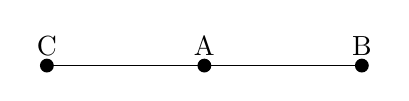
\begin{tikzpicture}
				\coordinate (A) at (0,0);
				\coordinate (B) at (2,0);
				\coordinate (C) at (-2,0);
				\draw (B) -- (C);
				%\draw [dashed] (M) -- (N);
				\node [above] at (A) {A};
				\node [above] at (B) {B};
				\node [above] at (C) {C};
				\fill (A) circle[radius=2.5pt];
				\fill (B) circle[radius=2.5pt];
				\fill (C) circle[radius=2.5pt];
			\end{tikzpicture}
		\end{center}

		\textbf{CÂU B} Sai vì $\overrightarrow{AB}-3\overrightarrow{AC}\Rightarrow \overrightarrow{CB}=-4\overrightarrow{AC}$.

		\begin{center}
			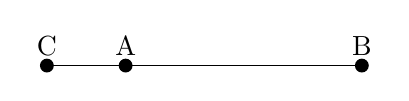
\begin{tikzpicture}
				\coordinate (A) at (-1,0);
				\coordinate (B) at (2,0);
				\coordinate (C) at (-2,0);
				\draw (B) -- (C);
				%\draw [dashed] (M) -- (N);
				\node [above] at (A) {A};
				\node [above] at (B) {B};
				\node [above] at (C) {C};
				\fill (A) circle[radius=2.5pt];
				\fill (B) circle[radius=2.5pt];
				\fill (C) circle[radius=2.5pt];
			\end{tikzpicture}
		\end{center}

		\textbf{CÂU C} Đúng theo định lý về sự đồng phẳng của 3 véctơ

		\textbf{CÂU D} Sai vì $\overrightarrow{AB}=3\overrightarrow{AC}\Rightarrow \overrightarrow{BA}=3\overrightarrow{CA}$ (nhân 2 vế cho $-1$)}
\end{ex}

\begin{ex}%[2H2N2-2]
	Trong không gian với hệ toạ độ $Oxyz$, cho điểm $A(3;-1;1)$. Hình chiếu vuông góc của điểm $A$ lên mặt phẳng $(Oyz)$ là điểm
	\choice
	{$M(3;0;0)$}
	{\True $N(0;-1;1)$}
	{$P(0;-1;0)$}
	{$Q(0;0;1)$}
	\loigiai{
		Khi chiếu vuông góc một điểm trong không gian lên mặt phẳng $(Oyz)$, ta giữ lại các thành phần tung độ và cao độ, còn hoành độ thì bằng $0$. Do đó, hình chiếu của $A(3;-1;1)$ lên $(Oyz)$ là điểm $N(0;-1;1)$.
	}
\end{ex}

\begin{ex}%[2H2H2-1]
	Trong không gian với hệ tọa độ $Oxyz$, cho hình hộp $ABCD\cdot A^{\prime} B^{\prime} C^{\prime} D^{\prime}$ có $A(0; 0; 0)$, $B(a; 0; 0)$, $D(0; 2a; 0)$, $A^{\prime}(0; 0; 2a)$ với $a \neq 0$. Độ dài đoạn thẳng $AC^{\prime}$ là
	\choice
	{$|a|$}
	{$2|a|$}
	{\True $3|a|$}
	{$\dfrac{3}{2}|a|$}
	\loigiai{
		\immini{Ta có $\overrightarrow{AB}=(a; 0; 0); \overrightarrow{AD}=(0; 2a; 0); \overrightarrow{AA^{\prime}}=(0; 0; 2a)$.\\
			Theo quy tắc hình hộp ta có \[\overrightarrow{AB}+\overrightarrow{AD}+\overrightarrow{AA^{\prime}}=\overrightarrow{AC^{\prime}} \Leftrightarrow \overrightarrow{AC^{\prime}}=(a; 2a; 2a).\]
			Suy ra $AC=|\overrightarrow{AC}|=\sqrt{a^2+(2a)^2+(2a)^2}=3|a|$.\\
			Vậy độ dài đoạn thẳng $AC^{\prime}=3|a|$.}{\begin{tikzpicture}[line cap=round, >=latex, scale=1]
				\def\a{3}
				\def\b{2}
				\def\h{3.5}
				\path 	(0:0) coordinate (A)
				++(0:\a) coordinate (D)
				++(-130:\b) coordinate (C)
				($(A)+(C)-(D)$) coordinate (B)
				($(A)+(90:\h)$) coordinate (A')
				($(B)+(90:\h)$) coordinate (B')
				($(C)+(90:\h)$) coordinate (C')
				($(D)+(90:\h)$) coordinate (D');
				\draw[dashed,thick] 	(B)--(A)--(D)	(A)--(A');
				\draw[thick] 	(C)--(C') 	(D)--(D') 	(B)--(B')	(C)--(C')
				(B)--(C)--(D)
				(A')--(B')--(C')--(D')--cycle;
				\foreach \x/\g in {A/180,B/180,C/0,D/0,A'/180,B'/180,C'/0,D'/0}
				\fill[black] 	(\x) circle (1pt)
				($(\g:4mm)+(\x)$) node {$\x$};
			\end{tikzpicture}}
	}
\end{ex}

\begin{ex}%[BG12 New, Anh Duy]%[2H2N2-4]
	Cho hai véc-tơ $\vec{a}=(1;-2;3)$ và $\vec{b}=(-2;1;2)$. Khi đó $\left(\vec{a}+\vec{b}\right)\vec{b}$ bằng
	\choice
	{$12 $}
	{$ 2$}
	{\True $ 11$}
	{$ 10$}
	\loigiai{
		Ta có $\vec{a}+\vec{b}=(-1;-1;5)$ nên $\left(\vec{a}+\vec{b}\right)\vec{b}=11$.
	}
\end{ex}

\begin{ex}%[2H2H2-1]
	Trong không gian với hệ tọa độ $Oxyz$, cho hình hộp $ABCD\cdot A^{\prime} B^{\prime} C^{\prime} D^{\prime}$ có $A(0; 0; 0)$, $B(a; 0; 0)$, $D(0; 2a; 0)$, $A^{\prime}(0; 0; 2a)$ với $a \neq 0$. Độ dài đoạn thẳng $AC^{\prime}$ là
	\choice
	{$|a|$}
	{$2|a|$}
	{\True $3|a|$}
	{$\dfrac{3}{2}|a|$}
	\loigiai{
		\immini{Ta có $\overrightarrow{AB}=(a; 0; 0); \overrightarrow{AD}=(0; 2a; 0); \overrightarrow{AA^{\prime}}=(0; 0; 2a)$.\\
			Theo quy tắc hình hộp ta có \[\overrightarrow{AB}+\overrightarrow{AD}+\overrightarrow{AA^{\prime}}=\overrightarrow{AC^{\prime}} \Leftrightarrow \overrightarrow{AC^{\prime}}=(a; 2a; 2a).\]
			Suy ra $AC=|\overrightarrow{AC}|=\sqrt{a^2+(2a)^2+(2a)^2}=3|a|$.\\
			Vậy độ dài đoạn thẳng $AC^{\prime}=3|a|$.}{\begin{tikzpicture}[line cap=round, >=latex, scale=1]
				\def\a{3}
				\def\b{2}
				\def\h{3.5}
				\path 	(0:0) coordinate (A)
				++(0:\a) coordinate (D)
				++(-130:\b) coordinate (C)
				($(A)+(C)-(D)$) coordinate (B)
				($(A)+(90:\h)$) coordinate (A')
				($(B)+(90:\h)$) coordinate (B')
				($(C)+(90:\h)$) coordinate (C')
				($(D)+(90:\h)$) coordinate (D');
				\draw[dashed,thick] 	(B)--(A)--(D)	(A)--(A');
				\draw[thick] 	(C)--(C') 	(D)--(D') 	(B)--(B')	(C)--(C')
				(B)--(C)--(D)
				(A')--(B')--(C')--(D')--cycle;
				\foreach \x/\g in {A/180,B/180,C/0,D/0,A'/180,B'/180,C'/0,D'/0}
				\fill[black] 	(\x) circle (1pt)
				($(\g:4mm)+(\x)$) node {$\x$};
			\end{tikzpicture}}
	}
\end{ex}

\begin{ex}%[2H2H2-4]
	Trong không gian $Oxyz$, cho hai điểm $A(2 ;-2 ; 1)$, $B(0 ; 1 ; 2)$. Tọa độ điểm $M$ thuộc mặt phẳng $(Oxy)$ sao cho ba điểm $A$, $B$, $M$ thẳng hàng là
	\choice
	{\True $M(4 ;-5 ; 0)$}
	{$M(2 ;-3 ; 0)$}
	{$M(0 ; 0 ; 1)$}
	{$M(4 ; 5 ; 0)$}
	\loigiai{
		Ta có $M \in(Oxy) \Rightarrow M(x ; y ; 0)$,  $\overrightarrow{AB}=(-2 ; 3 ; 1)$ ; $\overrightarrow{AM}=(x-2 ; y+2 ;-1)$.\\
		Để $A$, $B$, $M$ thẳng hàng thì $\overrightarrow{AB}$ và $\overrightarrow{AM}$ cùng phương.\\ Khi đó $\dfrac{x-2}{-2}=\dfrac{y+2}{3}=\dfrac{-1}{1} \Leftrightarrow\left\{\begin{array}{l}x=4 \\ y=-5.\end{array}\right.$\\
		Vậy $M(4 ;-5 ; 0)$.
	}
\end{ex}

\begin{ex}%[2H2V2-6]%[Dự án EX-TF-TLN NH 24-25-Vũ Hồng Toàn]
	\immini{
		Tính khoảng cách từ trọng tâm của một khối rubik (đồng chất) hình tứ diện đều đến một mặt của nó. Biết chiều cao của khối rubik là $8$ cm. (tham khảo hình vẽ bên)
	}{
		\begin{tikzpicture}[line join=round, line cap=round,>=stealth,declare function={a=4;g=40;b=2;h=3; }]
			\path (0,0) coordinate (A)++(0:a)coordinate (C)
			(-g:b) coordinate (B) ($(B)!.5!(C)$)coordinate (M)
			($(A)!2/3!(M)$)coordinate (H)++
			(90:h)coordinate (D);
			\draw[dash pattern=on 2pt off 1.5pt,thin] (C)--(A);
			\draw (D)--(A)--(B)--cycle--(C)--(B);
			\draw[|<->|,dash pattern=on 2pt off 1.5pt,thin] ($(H)+(0:3)$)--($(D)+(0:3)$)node[sloped,midway,fill=white, inner sep=1pt]{\footnotesize $8$ cm};
		\end{tikzpicture}
	}
	\choice
	{$4$ cm}
	{$3$ cm }
	{$1$ cm }
	{\True $2$ cm}
	\loigiai{
	\immini{
		Gọi $G$ và $I$ lần lượt là trọng tâm của tam giác $ABC$ và trọng tâm của khối rubik. Khi đó $IG=\mathrm{d}(I,(ABC))$.\\
		Ta có $\overrightarrow{DI} = 3\overrightarrow{IG} \Leftrightarrow \overrightarrow{IG} = \dfrac{1}{4}\overrightarrow{DG}$.\\
		Do đó $IG=\left|\overrightarrow{IG}\right| = \dfrac{1}{4}\left|\overrightarrow{DG}\right|=\dfrac{DG}{4}=2$.
		}{
			\begin{tikzpicture}[line join=round, line cap=round,>=stealth,declare function={a=4;g=40;b=2;h=3; }]
				\path (0,0) coordinate (A)++(0:a)coordinate (C)
				(-g:b) coordinate (B) ($(B)!.5!(C)$)coordinate (M)
				($(A)!2/3!(M)$)coordinate (G)++
				(90:h)coordinate (D) ($(D)!.75!(G)$)coordinate (I);
				\draw[dash pattern=on 2pt off 1.5pt,thin] (C)--(A) (D)--(G);
				\draw (D)--(A)--(B)--cycle--(C)--(B);
				\draw[|<->|,dash pattern=on 2pt off 1.5pt,thin] ($(G)+(0:3)$)--($(D)+(0:3)$)node[sloped,midway,fill=white, inner sep=1pt]{\footnotesize $8$ cm};
				\foreach \p/\g in {A/180,B/-90,C/0,D/90,G/0,I/0}
				\draw[fill=white] (\p) circle(1pt)+(\g:0.3) node{$\p$};
			\end{tikzpicture}
		}
	}
\end{ex}

\begin{ex}%[2D3N1-1]
	Cho bảng số liệu bên dưới. Hãy tính các tứ phân vị $Q_1$, $Q_2$, $Q_3$
	\begin{center}
		\begin{tabular}{|c|c|c|c|c|c|}
			\hline
			Nhóm   & $[46; 49)$ & $[49; 52)$ & $[52; 55)$ & $[55; 58)$ & $[58; 61)$ \\
			\hline
			Tần số & $18$       & $2$        & $13$       & $1$        & $6$        \\
			\hline
		\end{tabular}
	\end{center}
	\choice
	{$Q_1= 94; Q_2= 55; Q_3= 22$}
	{$Q_1= 61; Q_2= 33; Q_3= 22$}
	{\True $Q_1= 47{,}67; Q_2= 52; Q_3= 54{,}31$}
	{$Q_1= -39; Q_2= -11; Q_3= 22$}
	\loigiai{
		Áp dụng công thức tính tứ phân vị ta có
		\[Q_1= 47{,}67; Q_2= 52; Q_3= 54{,}31.\]
	}
\end{ex}

\begin{ex}%[2D3H1-2]
	Biểu đồ dưới đây thống kê thời gian tập thể dục buổi sáng mỗi ngày trong tháng 9/2022 của bác Bình và bác An.
	\begin{center}
		\begin{tikzpicture}[xscale=2,font=\footnotesize, line join=round, line cap=round, >=stealth]
			\draw[->](0,-0.2)--(0,7)node[left]{\textbf{Số ngày}};
			\draw[->](-0.2,0)--(6,0)node[below]{\textbf{phút}};
			\foreach \i in{1,...,6} \pgfmathsetmacro{\gti}{int(5*(\i))}
			\draw [dotted](0,\i) circle(1pt)node[left]{$\gti$} -- (5.5,\i);
			\foreach \i/\a/\b in {1/15/20,2/20/25,3/25/30,4/30/35,5/35/40}\draw (\i,0) node [below] {[\a;\b)};
			\foreach \i/\tr/\ph in {1/5/0,2/12/25,3/8/5,4/3/0,5/2/0}
				{
					\draw[fill=blue](\i,0)rectangle(\i-0.5,0.2*\tr) node [above right=0.3]{\tr};
					\draw[fill=orange](\i,0)rectangle(\i+0.5,0.2*\ph) node [above left=0.3]{\ph};
				}
			\foreach \i/\a/\b in {3/orange/Bác An, 4/blue/Bác Bình}
				{\draw (6,\i+1)node [right,fill=\a] {};
					\draw (6.2,\i+1) node[right]{\b};
				}
		\end{tikzpicture}
	\end{center}
	Khoảng biến thiên biểu thị thời gian tập thể dục của bác An là
	\choice
	{\True $10$ phút}
	{$15$ phút}
	{$20$ phút}
	{$25$ phút}
	\loigiai{
		Khoảng biến thiên của bác An là $R=30-20=10$ phút.
	}
\end{ex}

\begin{ex}%[2D3H1-3]
	Đo cân nặng của 1 lớp gồm $40$ học sinh lớp 12B ta được bảng số liệu sau
	\begin{center}
		\begin{tabular}{|c|c|c|c|c|c|c|c|c|}
			\hline
			Khối lượng (kg) & $[40;45)$ & $[45;50)$ & $[50;55)$ & $[55;60)$ & $[60;65)$ & $[65;70)$ & $[70;75)$ & $[75;80)$ \\
			\hline
			Số học sinh     & $4$       & $13$      & $7$       & $5$       & $6$       & $2$       & $1$       & $2$       \\
			\hline
		\end{tabular}
	\end{center}
	Tìm khoảng tứ phân vị của dãy số liệu trên.
	\choice
	{$15{,}5$}
	{\True $13{,}5$}
	{$15{,}3$}
	{$13{,}3$}
	\loigiai{
	Ta có
	\[
		Q_1=45+\dfrac{\dfrac{40}{4}-4}{13}\cdot 5\approx 47{,}3.
	\]
	\[
		Q_3=60+\dfrac{\dfrac{3\cdot 40}{4}-29}{6}\cdot 5\approx 60{,}8.
	\]
	Vậy khoảng tứ phân vị của mẫu số liệu trên là $\Delta Q=Q_3-Q_1=60{,}8-47{,}3=13{,}5$.
	}
\end{ex}

\begin{ex}%[2-D3B1-SO-3-2425]%[VN-MT-7-NguyenVanMinhHieu]%[2D3H1-4]
	Số lượng học sinh trên lớp đăng ký tham gia hoạt động Hoa phượng đỏ ở một trường THPT trên địa bàn TP.HCM được cho ở bảng sau:
	\begin{center}
		\begin{tabular}{|c|c|c|c|c|}
			\hline
			Điểm số     & $[6;10)$ & $[11;15)$ & $[16;20)$ & $[21;25)$ \\
			\hline
			Số học sinh & $4$      & $8$       & $2$       & $6$       \\
			\hline
		\end{tabular}
	\end{center}
	Giá trị nào sau đây là giá trị ngoại lệ của mẫu số liệu trên
	\choice
	{\True $38$}
	{$9$}
	{$15$}
	{$10$}
	\loigiai{
	Vì số học sinh là số nguyên nên ta hiệu chỉnh lại bảng số liệu sau
	\begin{center}
		\begin{tabular}{|c|c|c|c|c|}
			\hline
			Điểm số     & $[5{,}5;10{,}5)$ & $[10{,}5;15{,}5)$ & $[15{,}5;20{,}5)$ & $[20{,}5;25{,}5)$ \\
			\hline
			Số học sinh & $4$              & $8$               & $2$               & $6$               \\
			\hline
		\end{tabular}
	\end{center}
	Gọi $x_1$, $x_2$, $\ldots$, $x_{20}$ lần lượt là số điểm ghi được ở mỗi trận đấu xếp theo thứ tự không giảm.\\
	Tứ phân vị thứ nhất của mẫu số liệu là $\dfrac{1}{2}(x_5+x_6)$.\\
	Do $x_5$, $x_6 \in [10{,}5;15{,}5)$ nên tứ phân vị thứ nhất của mẫu số liệu nhóm là
	\[Q_1=10{,}5+\dfrac{\dfrac{20}{4}-4}{8}\cdot(15{,}5-10{,}5)=\dfrac{89}{8}= 11{,}125.\]
	Tứ phân vị thứ ba của mẫu số liệu là $\dfrac{1}{2}(x_{15}+x_{16})$.\\
	Do $x_{15}$, $x_{16} \in [20{,}5;25{,}5)$ nên tứ phân vị thứ ba của mẫu số liệu nhóm là
	\[Q_3=20{,}5+\dfrac{\dfrac{3\cdot 20}{4}-14}{6}\cdot(25{,}5-20{,}5)=\dfrac{64}{3}\approx 21{,}3.\]
	Khoảng tứ phân vị là $\Delta_Q=Q_3-Q_1=\dfrac{64}{3}-\dfrac{89}{8}=\dfrac{245}{24}\approx 10{,}21$.\\
	Suy ra $[Q_1-1{,}5\Delta_Q;Q_3+1{,}5\Delta_Q]\approx [-4{,}1875;36{,}65]$.\\
	Vậy giá trị ngoại lệ là $38$.
	}
\end{ex}
\begin{ex}%[2D3H2-1]
	Mẫu số liệu nào có độ phân tán lớn hơn thì
	\choice
	{phương sai và độ lệch chuẩn lớn hơn 1}
	{\True phương sai và độ lệch chuẩn càng lớn}
	{phương sai và độ lệch chuẩn bằng nhau}
	{độ lệch chuẩn bé hơn 0}
	\loigiai{Mẫu số liệu nào có độ phân tán lớn hơn thì phương sai và độ lệch chuẩn càng lớn.}
\end{ex}

\begin{ex}%[2-D3B2-SO-4-2425]%[VN-MT-7, Lư Phạm Minh Quân]%[2D3H2-2]
	Bảng dưới đây thống kê cân nặng của $45$ học sinh lớp $10$ của một trường Trung học phổ thông:
	\begin{center}
		\begin{tabular}{|c|c|c|}
			\hline
			Cân nặng (kg) & Số học sinh & Giá trị đại diện \\
			\hline
			$[40;44)$     & $8$         & $42$             \\
			\hline
			$[44;48)$     & $12$        & $46$             \\
			\hline
			$[48;52)$     & $8$         & $50$             \\
			\hline
			$[52;56)$     & $10$        & $54$             \\
			\hline
			$[56;60)$     & $7$         & $58$             \\
			\hline
			              & $n=45$      &                  \\
			\hline
		\end{tabular}
	\end{center}
	Độ lệch chuẩn của mẫu số liệu ghép nhóm là
	\choice
	{$1{,}15$}
	{\True $5{,}39$}
	{$2{,}15$}
	{$3{,}25$}
	\loigiai{
		Giá trị trung bình của mẫu số liệu ghép nhóm là
		\[\overline{x} = \dfrac{8\cdot 42 + 12\cdot 46 + 8\cdot 50 +10\cdot 54 + 7\cdot 58}{45} = \dfrac{2234}{45}.\]
		Phương sai của mẫu số liệu ghép nhóm là
		\[s^2 = \dfrac{1}{45} \left(8\cdot 42^2 + 12\cdot 46^2 + 8\cdot 50^2 +10\cdot 54^2 + 7\cdot 58^2\right) - \left(\dfrac{2234}{45}\right)^2 = \dfrac{58784}{2025} \approx 29{,}03.\]
		Độ lệch chuẩn của mẫu số liệu ghép nhóm là $s = \sqrt{\dfrac{58784}{2025}} \approx 5{,}39$.
	}
\end{ex}
\Closesolutionfile{ans}
\TL
\begin{bt} %[2D3H2-2] .
	Thống kê doanh thu (đơn vị: triệu đô la) của 20 công ty sản xuất ô tô trong năm 2023, người ta có bảng sau
	\begin{longtable}{|>{\centering\arraybackslash}p{2.5cm}|>{\centering\arraybackslash}p{2cm}|>{\centering\arraybackslash}p{2cm}|>{\centering\arraybackslash}p{2cm}|>{\centering\arraybackslash}p{2cm}|>{\centering\arraybackslash}p{2cm}|}
		\hline
		Doanh thu  & $[0;20)$ & $[20;40)$ & $[40;60)$ & $[60;80)$ & $[80;100]$ \\ \hline
		Số công ty & $5$      & $5$       & $6$       & $2$       & $2$        \\ \hline
	\end{longtable}
	\noindent Tính độ lệch chuẩn của mẫu số liệu ghép nhóm trên (kết quả làm tròn đến hàng phần chục).
	\loigiai{
		\begin{itemize}
			\item Chọn giá trị đại diện cho mẫu số liệu, ta có
			      \begin{longtable}{|>{\centering\arraybackslash}p{3cm}|>{\centering\arraybackslash}p{2cm}|>{\centering\arraybackslash}p{2cm}|>{\centering\arraybackslash}p{2cm}|>{\centering\arraybackslash}p{2cm}|>{\centering\arraybackslash}p{2cm}|}
				      \hline
				      Doanh thu        & $[0;20)$ & $[20;40)$ & $[40;60)$ & $[60;80)$ & $[80;100]$ \\ \hline
				      Giá trị đại diện & $10$     & $30$      & $50$      & $70$      & $90$       \\ \hline
				      Số công ty       & $5$      & $5$       & $6$       & $2$       & $2$        \\ \hline
			      \end{longtable}
			\item 	Điểm trung bình là
			      \[\overline{x}=\dfrac{5\cdot 10+5\cdot 30+6\cdot 50+2\cdot 70+2\cdot 90}{20}=41.\]
			\item 	Phương sai là
			      \[S^2=\dfrac{1}{20}\left[ 5\cdot  10^2+5\cdot 30^2+6\cdot 50 ^2+2\cdot  70^2+2\cdot  90^2 \right]- 41^2=619.\]
			\item	Độ lệch chuẩn: $S=\sqrt {619}\approx 24{,}9$.
		\end{itemize}}
\end{bt}

\begin{bt}%[2D1H5-8]
	Một chất điểm chuyển động theo quy luật $s(t)=-t^3+2t^2-t$, với $t$ (đơn vị: giây) là khoảng thời gian tính từ khi vật bắt đầu chuyển động và $s$ (đơn vị: mét) là quãng đường chất điểm di chuyển được trong khoảng thời gian đó. Trong khoảng thời gian $2$ giây kể từ khi bắt đầu chuyển động, chất điểm đạt được vận tốc lớn nhất là bao nhiêu?
	\loigiai{
		Ta có $v(t)=s'(t)=-3t^2+4t-1$, suy ra $v'(t)=-6t+4=0\Leftrightarrow t=\dfrac{2}{3}<2$.\\
		Ta có bảng biến thiên
		\begin{center}
			
\begin{tikzpicture}
				\tkzTabInit[nocadre=false,lgt=1.2,espcl=2.5,deltacl=0.6]
				{$t$/0.6, $v’(t)$/0.6, $v(t)$/2} % cột đầu tiên
				{$0$, $\tfrac{2}{3}$, $2$} % hàng 1 cột 2
				\tkzTabLine{,+,0,-,} % hàng 2 cột 2
				\tkzTabVar{-/ , +/ $\tfrac{1}{3}$ , -/ } % hàng 3 cột 2
			\end{tikzpicture}
		\end{center}
		Dựa vào bảng biến thiên, vận tốc đạt giá trị lớn nhất là $\dfrac{1}{3}$ khi $t=\dfrac{2}{3}$.
	}
\end{bt}

\begin{bt}%[2H2V2-6]
	Một người đứng ở mặt đất điều khiển hai flycam để phục vụ một chương trình của đài truyền hình. Flycam $I$ ở vị trí $A$ cách vị trí điều khiển $150\rm\,m$ về phía nam và $200\rm\,m$ về phía đông, đồng thời cách mặt đất $50\rm\,m$. Flycam $II$ ở vị trí $B$ cách vị trí điều khiển $180\rm\,m$ về phía bắc và $240\rm\,m$ về phía tây, đồng thời cách mặt đất $60\rm\,m$.\\
	Chọn hệ trục toạ độ $Oxyz$ với gốc $O$ là vị trí người điều khiển, mặt phẳng $(Oxy)$ trùng với mặt đất, trục $Ox$ có hướng trùng với hướng nam, trục $Oy$ có hướng trùng với hướng đông, trục $Oz$ vuông góc với mặt đất hướng lên bầu trời, đơn vị trên mỗi trục tính theo mét. Khoảng cách giữa hai flycam đó bằng bao nhiêu mét (làm tròn kết quả đến hàng đơn vị)?
	\loigiai{
		Flycam $I$ ở toạ độ $A(150;200;50)$.\\
		Flycam $II$ ở toạ độ $B(-180;-240;60)$.\\
		Khoảng cách gữa hai flycam bằng đoạn $AB$.\\
		Công thức tính khoảng cách đoạn thẳng. $AB=\sqrt{\left(x_B-x_A\right)^2+\left(y_B-y_A\right)^2+\left(z_B-z_A\right)^2}$\\
		Khoảng cách bằng $AB=\sqrt{\left(-180-150\right)^2+\left(-240-200\right)^2+\left(60-50\right)^2} =\sqrt{302600}\approx 550\rm\,m$.
	}
\end{bt}

\begin{bt}%[2D1C5-8]%[Dự án EX-TF-TLN-2024 - Đợt 2]%[Thành Đức Trung]
Trong đợt chào mừng kỉ niệm ngày 26 tháng 3, trường X có tổ chức cho các lớp bày các gian hàng tại sân trường. Để có thể che nắng, chứa đồ đạc trong quá trình tham gia hoạt động, một lớp đã nghĩ ra ý tưởng như sau: Dựng trên mặt đất bằng phẳng một chiếc lều từ một tấm bạt hình chữ nhật có chiều rộng là $4$ m và chiều dài là $6$ m, bằng cách gập đôi tấm bạt lại theo đoạn nối trung điểm hai cạnh là chiều dài của tấm bạt, hai mép chiều rộng còn lại của tấm bạt sát đất và cách nhau $x$ (m). Tìm giá trị của $x$ để khoảng không gian phía trong lều là lớn nhất.
\begin{center}
	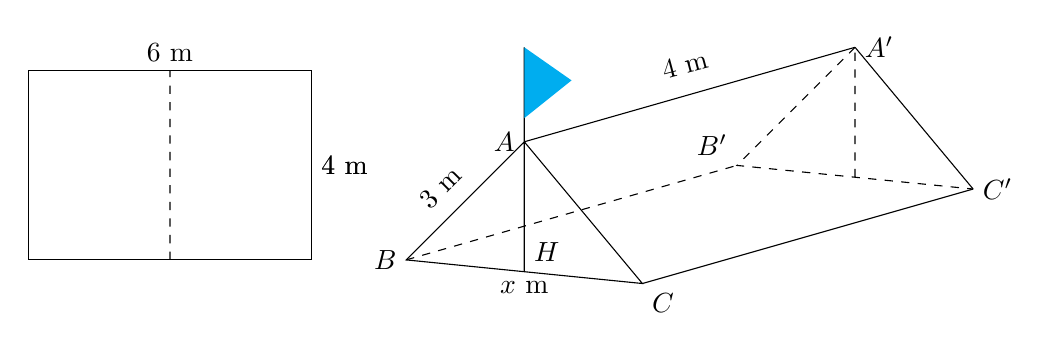
\begin{tikzpicture}[line cap=butt,line join=miter,>=stealth,scale=0.6]
		\draw (0,0)--(6,0)--(6,4)--(0,4)--cycle;
		\draw (8,0)--(13,-0.5)--(10.5,2.5)--cycle (20,1.5)--(17.5,4.5) (13,-0.5)--(20,1.5) (10.5,2.5)--(17.5,4.5) (10.5,-0.25)--(10.5,4.5);
		\draw[dashed] (17.5,4.5)--(15,2)--(20,1.5) (8,0)--(15,2) (17.5,1.75)--(17.5,4.5) (3,0)--(3,4);
		\fill[cyan](10.5,4.5)--(11.5,3.8)--(10.5,3)--cycle;
		\node at (6,2)[right]{$4$ m};
		\node at (3,4)[above]{$6$ m};
		\node at (6,2)[right]{$4$ m};
		\node at (10.5,2.5)[left]{$A$};
		\node at (8,0)[left]{$B$};
		\node at (13,-0.5)[below right]{$C$};
		\node at (17.5,4.5)[right]{$A'$};
		\node at (15,2)[above left]{$B'$};
		\node at (20,1.5)[right]{$C'$};
		\node at (10.5,-0.25)[below]{$x$ m};
		\node at (10.5,-0.25)[above right]{$H$};
		\node at (14,3.75)[rotate=15,above]{$4$ m};
		\node at (9,1.25)[rotate=45,above]{$3$ m};
		%		\node at (7,-2.5) [right,fill=white,font=\footnotesize]{\it Hình 1.38};
	\end{tikzpicture}
\end{center}
\loigiai{
Theo đề bài, ta có $0<x<6$.\\
Gọi tên như hình vẽ với $AH \perp BC$, suy ra $H$ là trung điểm của $BC$ nên $BH=\dfrac{BC}{2}=\dfrac{x}{2}$.\\
Xét tam giác $AHB$ vuông tại $B$, theo định lý\\
$AH=\sqrt{AB^2-BH^2}=\sqrt{3^2-\dfrac{x^2}{4}}=\dfrac{\sqrt{36-x^2}}{2}$.\\
$V_{ABC.A'B'C'}=S_{ABC}\cdot AA'=\dfrac{1}{2}AH\cdot BC\cdot AA'=\dfrac{1}{2}\cdot\dfrac{\sqrt{36-x^2}}{2}\cdot x\cdot 4=x\sqrt{36-x^2}$.\\
$V'=\sqrt{36-x^2}+x\cdot\dfrac{-2x}{2\sqrt{36-x^2}}=\sqrt{36-x^2}-\dfrac{x^2}{\sqrt{36-x^2}}=\dfrac{36-2x^2}{\sqrt{36-x^2}}$.\\
$V'=0\Leftrightarrow 36-2x^2=0\Leftrightarrow x=3\sqrt{2}$ hoặc $x=-3\sqrt{2}$ (loại).\\
Bảng biến thiên:
\begin{center}
	\begin{tikzpicture}[font=\normalsize,t style/.style={style=solid}]
		%dòng khai báo
		\tkzTabInit[lgt=1.2,espcl=3,deltacl=0.7]
		{$x$ /0.75, $V^{\prime}(x)$/0.75, $V(x)$/2.5}
		{$ 0$,$ 3\sqrt{2} $,$ 6 $}
		%dòng xét dấu
		\tkzTabLine{ , +,0 , -,} % z, t, d;
		%dòng biến thiên
		\path ($(N12)!0.8!(N13)$) node (A1){$0 $}
		($(N22)!0.2!(N23)$) node (A2){$ 18 $}
		($(N32)!0.8!(N33)$) node (A3){$ 0 $};
		\foreach \x/\y in {A1/A2,A2/A3}{
				\draw[-stealth] (\x)--(\y);
			}
	\end{tikzpicture}
\end{center}
Dựa vào bảng biến thiên, $x=3\sqrt{2}$ (m) thì khoảng không gian phía trong lều là lớn nhất.
}
\end{bt}
% \label{De5}
% %
% \cleardoublepage
% \setcounter{page}{1}
% \rfoot{Trang \thepage/\pageref{DA5} - Đáp án trắc nghiệm Đề 5}
% \begin{center}
% 	\bfseries ĐÁP ÁN TRẮC NGHIỆM ĐỀ 5
% \end{center}

% \inputansbox{10}{ans/ansDe5-TN5}
% \label{DA6}
% %
